\documentclass[11pt]{article}

\input{../../preamble.tex}

\usepackage[margin=1in]{geometry}
\usepackage{amsmath,amssymb,bm}
\usepackage{graphicx}
\usepackage{float}
\usepackage{setspace}

% ---------- Small helpers ----------
\newcommand{\kb}[1]{\bm{k}_{#1}}
\newcommand{\ob}[1]{\bm{o}_{#1}}
\newcommand{\vb}{\bm{v}}
\newcommand{\wb}{\bm{\omega}}
\newcommand{\J}{\bm{J}}
\newcommand{\q}{\bm{q}}
\newcommand{\qd}{\dot{\bm{q}}}
\newcommand{\twist}{\begin{bmatrix}\vb\\ \wb\end{bmatrix}}

\begin{document}
\thispagestyle{empty}

% =======================
% Header (match handout)
% =======================
\begin{center}
{\large University of British Columbia}\\
{\large Department of Electrical \& Computer Engineering}\\
{\large MECH 464/563\ \ EECE 442/589: Introduction to Robotics}\\[4pt]
{\large Assignment \#4}\\
Dominic Klukas\\
SN: 64348378
\end{center}

\vspace{0.75em}

% =======================
% Prompt text (match handout)
% =======================
Read Chapter 3 from my notes (ch3\_velkin.pdf), Corke, Sec.\ 8.1.4, 8.2.1, 8.2.2 (Jacobian singularities).\\
Find the manipulator geometric Jacobian for the robots shown in Figures 1, 2 and 3.\\
For each case, find the robot singular configurations.

\vspace{1.25em}

% =======================
% Figures (match captions)
% =======================
\begin{figure}[H]
  \centering
  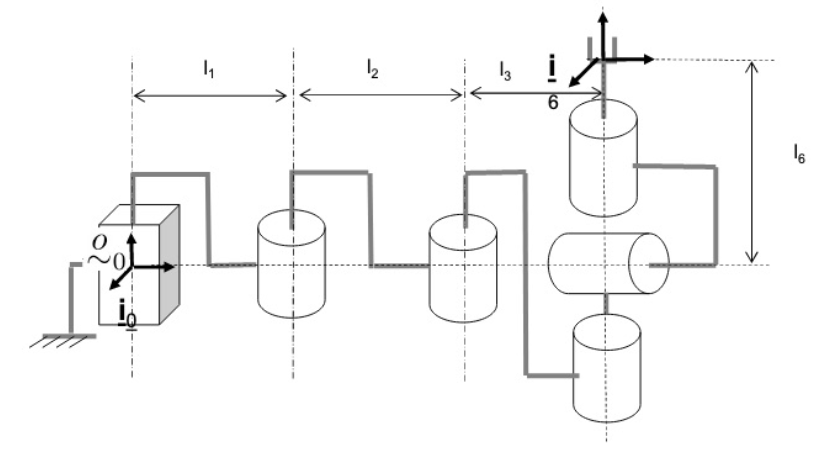
\includegraphics[width=0.62\linewidth]{SCARA.png}
  \caption{SCARA robot with vertical axis in the base.}
\end{figure}

\begin{figure}[H]
  \centering
  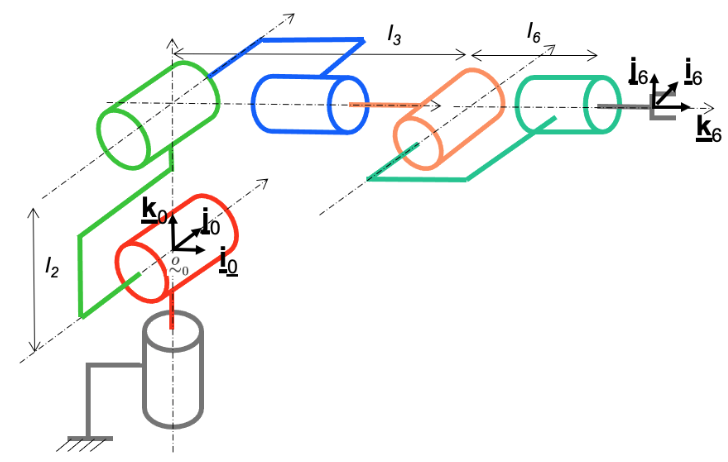
\includegraphics[width=0.70\linewidth]{PUMA_nooffset.png}
  \caption{Anthropomorphic (PUMA without offsets).}
\end{figure}

\begin{figure}[H]
  \centering
  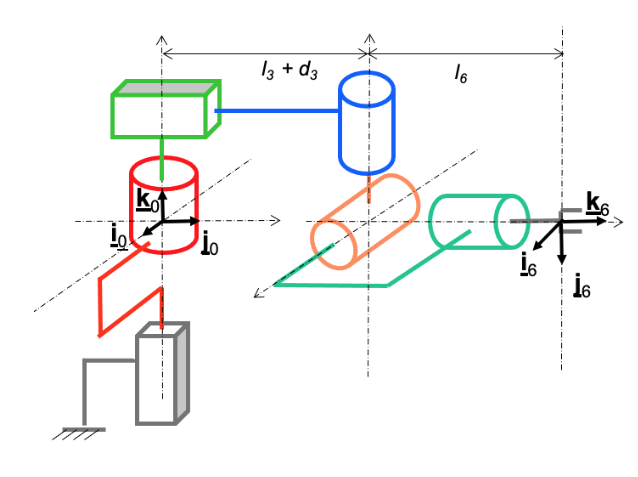
\includegraphics[width=0.70\linewidth]{CylindricalRobot.png}
  \caption{Cylindrical robot.}
\end{figure}

\newpage
\setcounter{page}{1}

% ==========================================================
% ================   YOUR SOLUTION STARTS   =================
% ==========================================================


\section{Figure 1: SCARA}
Given that the first joint is prismatic and the rest are revolute, we have that the geometric Jacobian is
\[
    J = \begin{bmatrix} k_0 & k_1 \times (o_6 - o_1) &  k_2 \times (o_6 - o_2) &  k_3 \times (o_6 - o_3) & k_4 \times (o_6 - o_4) &  k_5 \times (o_6 - o_5) \\ 0 & k_1 & k_2 & k_3 & k_4 & k_5 \end{bmatrix} 
.\] 

However, by the DH convention, we would have that the co-ordinate origins for $o_3$, $o_4$, and $o_5$ are coincident, because the axes of those three joints pass through each other.
Also, we have that $k_0, k_1, k_2$ are the same unit vector, so we simplify, to get the geometric jacobian:

\[
    J = \begin{bmatrix} k_0 & k_0 \times (o_6 - o_1) &  k_0 \times (o_6 - o_2) &  k_3 \times (o_6 - o_3) & k_4 \times (o_6 - o_3) &  k_5 \times (o_6 - o_3) \\ 0 & k_0 & k_0 & k_3 & k_4 & k_5 \end{bmatrix} 
.\] 

Finally, to expose the singular configurations, we multiply (on the left) by a matrix with determinant one, which will not change the singularity of the resulting product:
\[
    \begin{bmatrix} I_{3 \times  3} & (o_6 - o_3) \times \\ 0 & I_{3 \times  3} \end{bmatrix}  J = \begin{bmatrix} k_0 & k_0 \times (o_3 - o_1) & k_0 \times  (o_3 - o_2) & 0 & 0 & 0\\ 0 & k_0 & k_0 & k_3 & k_4 & k_5  \end{bmatrix} 
.\] 
We analyze the singularity conditions:
\begin{itemize}
    \item  Analyzing the diagram, we can see that $k_4 \perp k_3$ and $k_4 \perp k_5$ at all times. However, we have the possibility that $k_3 \parallel k_5$, in which case the matrix is singular.
        This corresponds to a gimbal lock in the spherical wrist.
    \item 
        We have by default that $k_0 \perp k_0 \times (o_3 - o_{1, 2})$, so for the velocity components to cause a non-singularity, we would require $(o_3 - o_1) \parallel (o_3 - o_2)$.
        That happens, for instance, when both joints 2 and 3 are fully extended.
\end{itemize}


\section{Figure 2: PUMA without offsets}

We have that all the joints are revolute, giving us a Jacobian of the form:
\[
    J = \begin{bmatrix} k_0 \times (o_6 - o_0)  & k_1 \times (o_6 - o_1) &  k_2 \times (o_6 - o_2) &  k_3 \times (o_6 - o_3) & k_4 \times (o_6 - o_4) &  k_5 \times (o_6 - o_5) \\ k_0 & k_1 & k_2 & k_3 & k_4 & k_5 \end{bmatrix} 
.\] 

However, if we follow the DH convention we have that $k_1 = k_2$, $o_0 = o_1$ and $o_3 = o_4 = o_5$, so we can simplify:

\[
    J = \begin{bmatrix} k_0 \times (o_6 - o_0)  & k_1 \times (o_6 - o_0) &  k_1 \times (o_6 - o_2) &  k_3 \times (o_6 - o_3) & k_4 \times (o_6 - o_3) &  k_5 \times (o_6 - o_3) \\ k_0 & k_1 & k_1 & k_3 & k_4 & k_5 \end{bmatrix} 
.\] 


Finally, to find the singularities, we use the fact that we have a spherical wrist by premultiplying with a matrix of determinant 1:
\[
    \begin{bmatrix} I_{3 \times  3} & (o_6 - o_3) \times \\ 0 & I_{3 \times  3} \end{bmatrix}  J  = \begin{bmatrix} k_0 \times (o_3 - o_0)  & k_1 \times (o_3 - o_0) &  k_1 \times (o_3 - o_2) & 0 & 0 & 0  \\ k_0 & k_1 & k_1 & k_3 & k_4 & k_5 \end{bmatrix} 
.\] 

Then, we observe the singularities:
\begin{itemize}
    \item Like last time, we observe from the diagram that $k_3 \perp k_4$ and $k_4 \perp k_5$, but we have the possibility, again, of gimbal lock, when $k_3 \parallel k_5$, causing a singularity.
    \item If $k_0 \parallel (o_3 - o_0)$, then $k_0 \times (o_3 - o_0) = 0$, and we have a singularity. This happens when the spherical wrist origin $o_3=o_4=o_5$ than axis 1.
    \item If $(o_3 - o_0) \parallel (o_3 - o_2)$, then we also have a singularity because then we have two linearly dependent columns.
\end{itemize}

\section{Figure 3: Cylindrical robot}

The first and third joints are prismatic and the rest are revolute, with a spherical wrist.
With the DH co-ordinates, we can choose $o_0 = o_1 = o_2$ to be at the co-ordinate frame $o_0$.
Then, we have the geometric jacobian:
\[
    J = \begin{bmatrix} k_0 & k_1 \times (o_6 - o_1) & k_2 & k_3 \times (o_6 - o_3) & k_4 \times (o_6 - o_4) & k_5 \times (o_6 - o_5) \\ 0 & k_1 & 0 & k_3 & k_4 & k_5 \end{bmatrix} 
.\] 

For the singularities, we use the the spherical wrist:
\[
    J = \begin{bmatrix} k_0 & k_1 \times (o_3 - o_1) & k_2 & 0  & 0 & 0 \\ 0 & k_1 & 0 & k_3 & k_4 & k_5 \end{bmatrix} 
.\] 
\begin{itemize}
    \item $k_3 \parallel k_5$ gives us a singularity as a result of a gimbal lock in the spherical wrist.
    \item Two prismatic joints in the shoulder gives us no other singularities.
\end{itemize}
\end{document}
